\chapter{Nexys 4 DDR}

\begin{figure}[H]
  \centering
  \includegraphics[width=0.70\textwidth]{images/nexys_4_ddr.png}
  \caption{Image of the Nexis 4 DDR board with the elements used in the project highlighted.}
  \label{fig:nexys_4_ddr}
\end{figure}

One of the objectives of this project is to provide an interaction between the Nexys 4 DDR board and the previously developed hardware modules, in particular the CORDIC unit. The board is used as a simple hardware calculator for computing the sine and cosine of a given angle. The user selects the input angle in binary format through the on-board switches and chooses whether to compute the sine or the cosine. Once the input has been configured, the computation is triggered by pressing a push button. The CORDIC module then performs the calculation, and the resulting value is displayed on the seven-segment display available on the board.

This chapter describes all the hardware and control elements required to enable this interaction, including the input interface, the control logic, and the output visualization on the Nexys 4 DDR platform.

\pagebreak
\section{Constraints File}

In order to ensure proper communication between the hardware design and the physical Nexys 4 DDR board, it is necessary to define a constraints file. The constraints file (.xdc) specifies how the logical signals of the design are mapped to the physical pins of the FPGA device, enabling the interaction between the implemented hardware modules and the external peripherals available on the board.

A reference template of the constraints file for the Nexys 4 DDR board is provided by Digilent on \href{https://github.com/Digilent/Nexys-4-DDR-OOB/blob/master/src/constraints/Nexys4DDR_C.xdc}{GitHub}. This template can be used as a starting point and adapted to the specific requirements of the project.

For this project, only a subset of the available I/O resources is required. In particular, the signals used to interface with push buttons, LEDs, switches, and the seven-segment display have been constrained and mapped to the corresponding physical pins of the board.

\pagebreak
\section{Debouncer and Pulse Generator}

\begin{figure}[H]
  \centering
  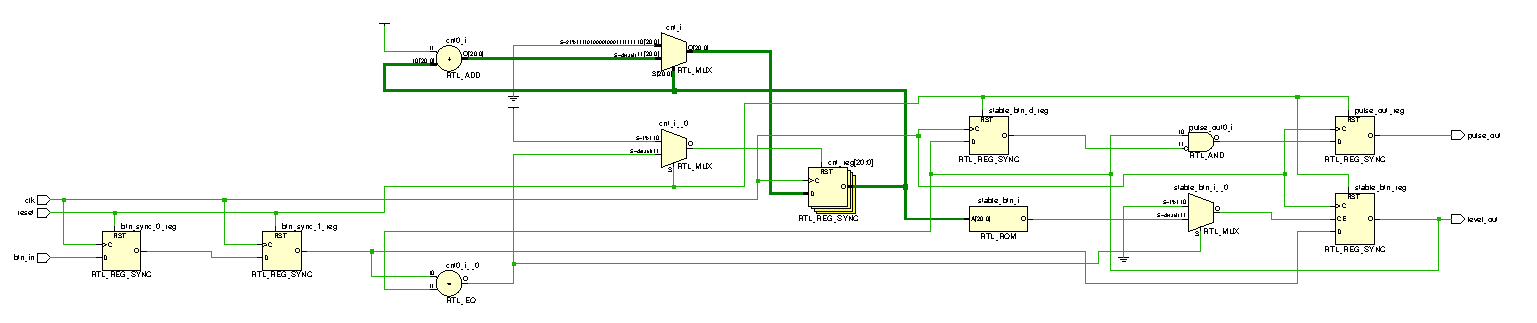
\includegraphics[width=\textwidth]{images/debouncer.pdf}
  \caption{High-level overview of the Debouncer and Pulse Generator module as rendered by Vivado.}
  \label{fig:debouncer}
\end{figure}

Mechanical pushbuttons produce noisy signals due to contact bouncing and are not synchronized with the system clock. For this reason, their raw output cannot be used directly to control synchronous hardware modules. The Debouncer and Pulse Generator module provides a clean and reliable interface between the pushbutton inputs of the Nexys 4 DDR board and the digital logic of the system.

The module first synchronizes the asynchronous button signal to the system clock using a two-stage flip-flop synchronizer, reducing the risk of metastability. The synchronized signal is then filtered by a debounce mechanism based on a counter. A new button state is accepted only if the input remains stable for a configurable number of clock cycles, defined by the debounce window parameter. This ensures that short glitches caused by mechanical bouncing are ignored.

Once a stable button level has been detected, a rising-edge detector generates a single-clock-wide pulse whenever the button is pressed. This pulse is suitable for triggering control actions, such as starting a CORDIC computation, without the risk of multiple activations caused by a prolonged button press. In addition to the pulse signal, the module also provides the debounced button level, which can be used for monitoring or control purposes if required.

This module plays a key role in ensuring reliable user interaction with the system, as it guarantees that each physical button press results in a single, well-defined control event.

\pagebreak
\section{7-Segment Display Driver}

\begin{figure}[H]
  \centering
  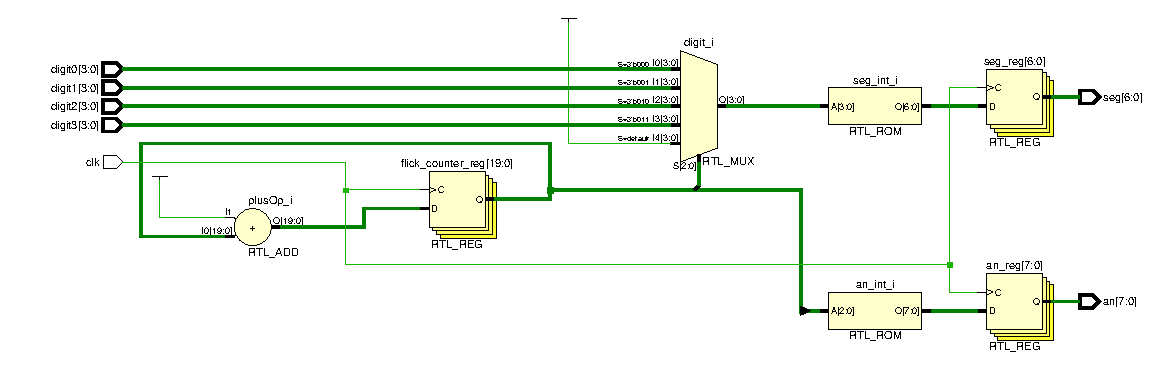
\includegraphics[width=\textwidth]{images/seven_seg_driver.pdf}
  \caption{High-level overview of the 7-Sefmante Display driver as rendered by Vivado.}
  \label{fig:seven_seg_driver}
\end{figure}

In order to correctly visualize numerical values on the seven-segment display of the Nexys 4 DDR board, the output signals generated by the hardware modules must be properly encoded. The 7-segment display driver is responsible for translating a binary digit into the corresponding pattern of segments to be activated on the display.

Each digit to be shown is mapped to a specific combination of the seven LED segments. This mapping is defined through a combinational encoding table, where each possible input value is associated with the corresponding segment activation pattern. The driver therefore acts as an interface between the binary representation of a number and its human-readable visualization on the display.

Listing~\ref{lst:sevenseg_encoding} shows an example of the encoding logic used to map a 4-bit digit to the corresponding seven-segment pattern. Invalid or unsupported input values are mapped to a blank display configuration.

{\scriptsize
\begin{lstlisting}[
    caption={Seven-segment display encoding table for decimal digits.},
    label={lst:sevenseg_encoding},
    breaklines=true,
    breakatwhitespace=true,
    columns=flexible
]
with digit select
        seg_int <=
            "1000000" when "0000", -- 0
            "1111001" when "0001", -- 1
            "0100100" when "0010", -- 2
            "0110000" when "0011", -- 3
            "0011001" when "0100", -- 4
            "0010010" when "0101", -- 5
            "0000010" when "0110", -- 6
            "1111000" when "0111", -- 7
            "0000000" when "1000", -- 8
            "0010000" when "1001", -- 9
            "1111111" when others; -- blank / invalid
\end{lstlisting}
}

\begin{figure}[H]
  \centering
  \includegraphics[width=\textwidth]{images/display.png}
  \caption{Example of the seven-segment display encoding for decimal digits.}
  \label{fig:display}
\end{figure}

This encoding approach allows the display driver to present the computed results of the CORDIC module in a clear and readable format, enabling direct visual feedback to the user through the on-board display.

\pagebreak
\section{Top Level for Nexys 4 DDR}

The top-level module represents the integration layer between the board-specific interface logic and the CORDIC computation modules. Its main purpose is to interconnect the input and output peripherals of the Nexys 4 DDR board with the internal hardware components responsible for the computation and control flow.

This module instantiates and connects the CORDIC core, the input handling logic (including debouncers and control signals derived from pushbuttons and switches), and the output interface modules used to drive the LEDs and the seven-segment display. As a result, it acts as the main coordination point of the system, ensuring that user inputs are correctly interpreted and that the computed results are properly visualized on the board.

Listing~\ref{lst:top_nexys_entity} reports the entity declaration of the top-level module used for the Nexys 4 DDR board. The interface exposes the board clock, the user input signals, and the output signals required to drive the on-board peripherals.

{\scriptsize
\begin{lstlisting}[
    caption={Entity declaration of the Nexys 4 DDR top-level module.},
    label={lst:top_nexys_entity},
    breaklines=true,
    breakatwhitespace=true,
    columns=flexible
]
entity top_nexys is
    generic (
        WIDTH      : integer := 16;
        ITERATIONS : integer := 16
    );
    port (
        -- Clock from Nexys4 DDR (100 MHz)
        clk100mhz : in  std_logic;

        -- User inputs
        sw  : in  std_logic_vector(15 downto 0);  -- switches
        btn : in  std_logic_vector(4 downto 0);   -- pushbuttons

        -- User outputs
        led : out std_logic_vector(15 downto 0);  -- LEDs
        an  : out std_logic_vector(7 downto 0);   -- 7-seg anodes (active low)
        seg : out std_logic_vector(6 downto 0)    -- 7-seg segments (g..a, active low)
    );
end top_nexys;
\end{lstlisting}
}

This top-level organization enables a clear separation between board-specific interfaces and computational logic, simplifying both verification and future extensions of the system.

\pagebreak
\section{Interaction with Nexys 4 DDR}

Once the board has been programmed, it is possible to interact with the system through the on-board peripherals. The following elements of the Nexys 4 DDR board are used:

\begin{itemize}
    \item Switches from 0 to 8 are used to select the input angle in binary format. Since the selectable angles range from 0 to 359 degrees, the maximum value to be represented is 359 in decimal, corresponding to 101100111 in binary, which requires 9 bits.
    \item Switch 9 is used to select the trigonometric function: cosine when the switch is off and sine when the switch is on.
    \item The central pushbutton (BTNC, N17) is used to start the computation.
    \item The seven-segment display is used to show the computed result using four decimal digits. The displayed format is N.NNN, where the first digit represents the integer part and the remaining three digits represent the fractional part.
\end{itemize}

A schematic view of the board elements involved in the interaction and their corresponding roles is shown in Figure~\ref{fig:nexys_test}.

\begin{figure}[H]
  \centering
  \includegraphics[width=\textwidth]{images/nexys_test.png}
  \caption{Overview of the interactive elements on the Nexys 4 DDR board.}
  \label{fig:nexys_test}
\end{figure}

\pagebreak
Two experimental tests are reported below. In the first test, the sine of 35 degrees is evaluated. The value 35 is selected through the switches in binary form (100011), and switch 9 is set to select the sine function. The value shown on the display is 0.573, which is consistent with the expected result, since sin(35°) = 0.57357644. The sign LED remains off because the result is positive.

\begin{figure}[H]
  \centering
  \includegraphics[width=0.75\textwidth]{images/sin_35.png}
  \caption{Expected reult for sin(35°) on the Nexys 4 DDR board.}
  \label{fig:sin_35}
\end{figure}

\begin{figure}[H]
  \centering
  \includegraphics[width=0.75\textwidth]{images/sin_35_irl.jpg}
  \caption{Hardware test of sin(35°) on the Nexys 4 DDR board.}
  \label{fig:sin_35_irl}
\end{figure}

In the second test, the cosine of 130 degrees is evaluated. The value 130 is selected through the switches in binary form (10000010), and switch 9 is set to select the cosine function. The value shown on the display is 0.642, which matches the expected magnitude of the result, since cos(130°) = -0.64278761. In this case, the sign LED is turned on to indicate that the computed value is negative.

\begin{figure}[H]
  \centering
  \includegraphics[width=0.75\textwidth]{images/cos_130.png}
  \caption{Expected result for cos(130°) on the Nexys 4 DDR board.}
  \label{fig:cos_130}
\end{figure}

\begin{figure}[H]
  \centering
  \includegraphics[width=0.75\textwidth]{images/cos_130_irl.jpg}
  \caption{Hardware test of cos(130°) on the Nexys 4 DDR board.}
  \label{fig:cos_130_irl}
\end{figure}